\documentclass{beamer}

    \usepackage{xeCJK}

    \usetheme[progressbar=frametitle]{metropolis}
    \usepackage{appendixnumberbeamer}
    
    \usepackage{booktabs}
    \usepackage[scale=2]{ccicons}
    
    \usepackage{pgfplots}
    \usepgfplotslibrary{dateplot}
    
    \usepackage{xspace}
    \newcommand{\themename}{\textbf{\textsc{metropolis}}\xspace}
    
    \title{操作系统探索}
    %\subtitle{A modern beamer theme}
    % \date{\today}
    \date{2018年4月}
    \author{尹志成 \\ 指导教师:王晓林}
    \institute{西南林业大学大数据与智能工程学院}
    % \titlegraphic{\hfill\includegraphics[height=1.5cm]{logo.pdf}}
    
    \begin{document}

    \maketitle
    \begin{frame}{Table of contents}
      \setbeamertemplate{section in toc}[sections numbered]
      \tableofcontents[hideallsubsections]
    \end{frame}
    
    \section{技术路线}
    \begin{frame}[fragile]{技术路线}
        \begin{enumerate}
            \item 操作系统探究
            \item 编写操作系统内核
              \begin{enumerate}
                  \item 空白操作系统启动
                  \item 内存管理
                  \item 输入输出
                  \item 多道程序设计及分时系统
              \end{enumerate}
            \item 对外兼容及安全防护
        \end{enumerate}
    \end{frame}

    \section{操作系统探究}
    \begin{frame}{操作系统探究}
      \begin{figure}[H]
        \centering
        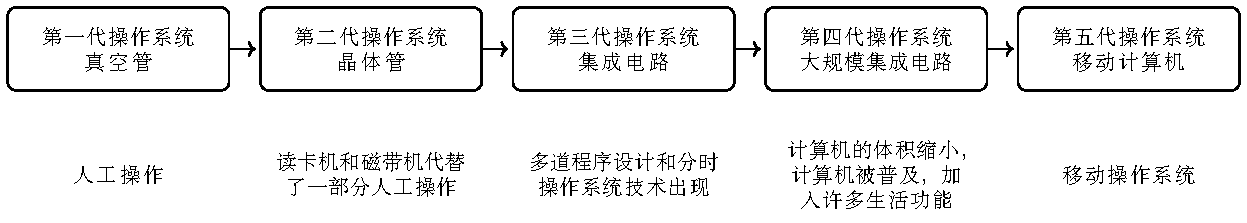
\includegraphics[width=\textwidth]{fig/explorer.pdf}
      \end{figure}
    \end{frame}

    \section{编写操作系统内核}
    \begin{frame}{整体设计}
      \begin{figure}[H]
        \centering
        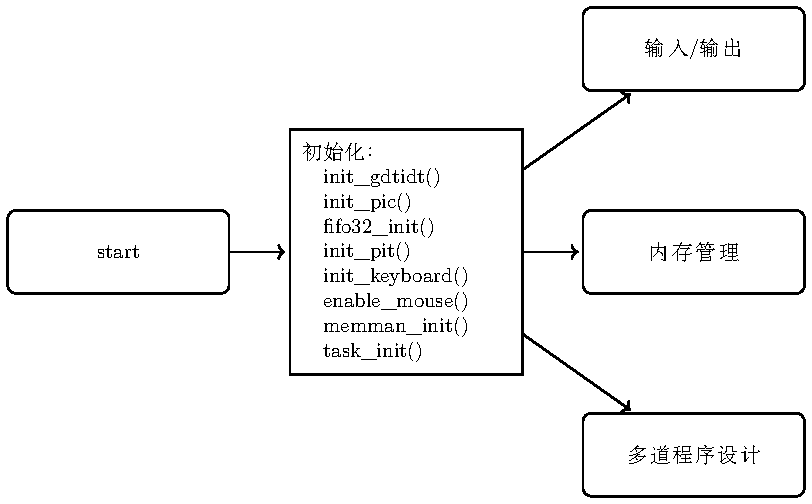
\includegraphics[width=\textwidth]{../../Thesis/fig/func/run.pdf}
      \end{figure}
    \end{frame}
    \begin{frame}{内存管理}
      \begin{figure}[H]
        \centering
        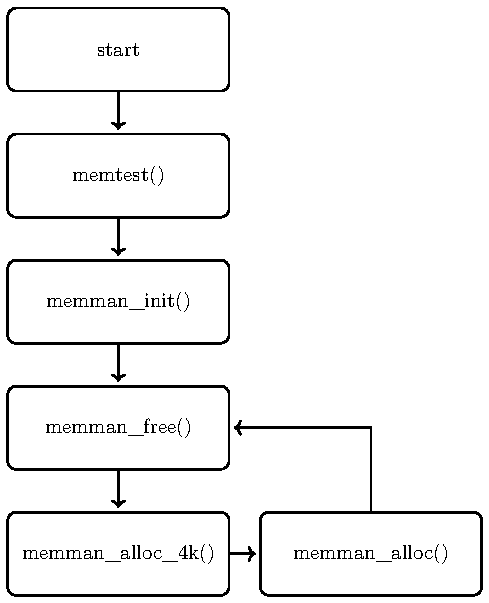
\includegraphics[width=.5\textwidth]{../../Thesis/fig/func/memman.pdf}
      \end{figure}
    \end{frame}
    \begin{frame}{输入输出}
      \begin{figure}[H]
        \centering
        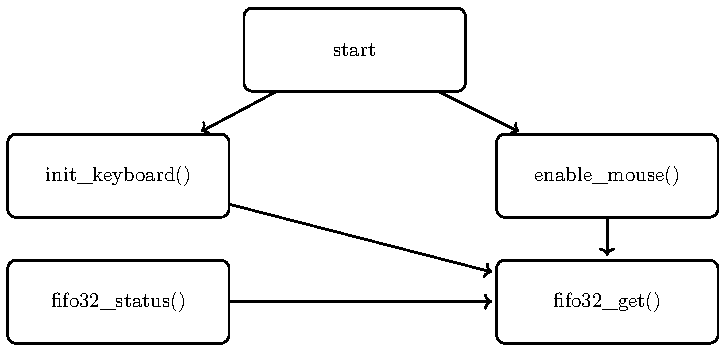
\includegraphics[width=\textwidth]{../../Thesis/fig/func/io.pdf}
      \end{figure}
    \end{frame}
    \begin{frame}{多道程序设计及分时操作系统}
      \begin{figure}[H]
        \centering
        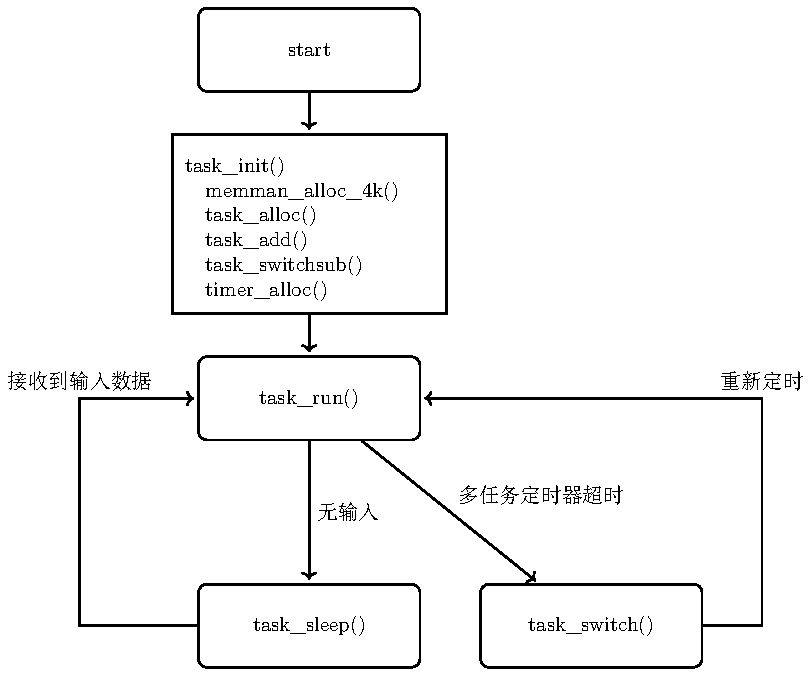
\includegraphics[width=.8\textwidth]{../../Thesis/fig/func/multi.pdf}
      \end{figure}
    \end{frame}
    
    \section{对外兼容及安全防护}
    
      \begin{frame}{对外兼容及安全防护}
        \begin{figure}[H]
          \centering
          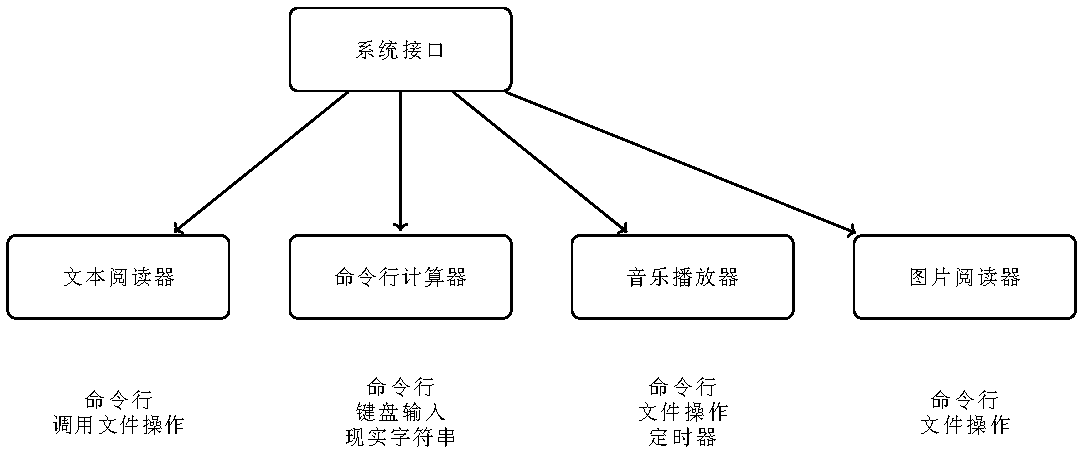
\includegraphics[width=.8\textwidth]{fig/sc.pdf}
        \end{figure}
      \end{frame}

    \begin{frame}{}
    
      THANKS FOR WATCHING!
      
    \end{frame}
    
    \end{document}